% !TEX encoding = UTF-8 Unicode


\documentclass[conference,compsoc]{IEEEtran}

\usepackage{microtype}

\usepackage[dvipsnames]{xcolor}
\usepackage{siunitx}
\usepackage{amsmath}
\usepackage{amsfonts}
\usepackage{amssymb}
\usepackage{csquotes}
\usepackage{array}
\newcolumntype{L}[1]{>{\raggedright\let\newline\\\arraybackslash\hspace{0pt}}m{#1}}
\newcolumntype{C}[1]{>{\centering\let\newline\\\arraybackslash\hspace{0pt}}m{#1}}
\newcolumntype{R}[1]{>{\raggedleft\let\newline\\\arraybackslash\hspace{0pt}}m{#1}}


\usepackage[utf8]{inputenc}
\usepackage[english]{babel}
\usepackage{pgfplots}
\usepackage{url}
\usepackage{hyperref} 
\usepackage{float}
\usepackage{tabularx,caption}
\usepackage{csvsimple}
\usepackage{listings,mdframed}



\usepackage[utf8]{inputenc}
\usepackage[english]{babel}

\usepackage{url}
\usepackage{hyperref} 
\usepackage{graphicx}
\usepackage{fancyref}
\usepackage{amsmath}

% *** CITATION PACKAGES ***
%
\ifCLASSOPTIONcompsoc
  % IEEE Computer Society needs nocompress option
  % requires cite.sty v4.0 or later (November 2003)
  \usepackage[nocompress]{cite}
\else
  % normal IEEE
  \usepackage{cite}
\fi

\begin{document}

\title{LU Factorisation with Partial Pivoting}


% author names and affiliations
% use a multiple column layout for up to three different
% affiliations
\author{\IEEEauthorblockN{Filipe Oliveira\IEEEauthorrefmark{1} and Sérgio Caldas\IEEEauthorrefmark{1}}
\IEEEauthorblockA{University of Minho\\ Computer Science Department\\
Email: \IEEEauthorrefmark{1}a57816@alunos.uminho.pt, \IEEEauthorrefmark{2}a57779@alunos.uminho.pt }
}


% make the title area
\maketitle

\begin{abstract}

In order to solve a linear system, the Gaussian eliminations with partial pivoting is one of the most efficient and accurate ways to do it.\par 
 In the absence of pivoting, the total error found on the final solution is sometimes undesired. 
A row-oriented implementation of Gaussian elimination with partial pivoting on a local-memory multiprocessor is described, and also a blocked row-oriented implementation of Gaussian elimination with partial pivoting. \par 

A simple error and total time to solution analysis is made, providing the comparison between LU factorisation with and without partial pivoting, and also the comparation between blocked and non-blocked versions.


\end{abstract}

% no keywords

\begin{IEEEkeywords} Gaussian elimination; Linear Algebra; multiprocessor; LU Factorisation\footnote{Lecture 12 LU Decomposition} ; Linear Systems Pivoting \end{IEEEkeywords}


\IEEEpeerreviewmaketitle



\section{Introduction}
\subsection{LU Factorisation without Partial Pivoting}
The LU Factorisation\footnote{LU Decomposition} is a method used to solve a linear system of equations. This factorisation uses two matrices, one upper matrix (triangular superior matrix) and a lower matrix (triangular inferior matrix). The LU Factorisation can be viewed as the matrix form of Gaussian elimination. A math definition for LU factorisation is:

\begin{displayquote}
Let A be a square matrix. An LU factorisation refers to the factorisation of A, with proper row and/or column orderings or permutations, into two factors, a lower triangular matrix L and an upper triangular matrix U.
\end{displayquote}

The equation that translate this definition is:

\begin{equation}
    A = LU
\end{equation}

In the lower matrix, all elements above the diagonal are zeros, in the upper matrix all elements below the diagonal are zeros and in the upper matrix all elements of diagonal are 1.

\subsection{LU Factorisation with Partial Pivoting}
In the LU Factorisation with Partial Pivoting, the factorisation refers often to the LU factorisation with row permutations only. The LU Factorisation can be defined for the following equation:

\begin{equation}
    PA = LU
\end{equation}

Where L and U, are the lower and the upper matrix respectively and P, refers to a permutation matrix. The permutation matrix, is a binary matrix where in each row and column only have one entry of 1, the others elements are zeros. When we multiply permutation matrix for other matrix, this produce the permutation in the rows or columns of the other matrix. 

\section{Hardware characterisation}

The computing platform, our team laptop, is a  Intel\textsuperscript{\textregistered} Core\textsuperscript{TM} i7-3635QM (Ivy Bridge architecture). The system features 16 GB of DDR3 RAM, supported at a frequency of 1600MHz, divided in 2 memory channels. \par 

The characteristics of the CPU on the computing platform is presented in the table \ref{table:characterisation}.

\begin{table}[H]
\centering
  \begin{tabular}{ | L{5cm} | R{2.2cm} |}
    \hline
    System &  team laptop \\ \hline \hline
        \# CPUs  & 1 \\ \hline
    CPU  & Intel\textsuperscript{\textregistered} Core\textsuperscript{TM} i7-3635QM \\ \hline 
    Architecture & Ivy Bridge \\ \hline 
    \# Cores per CPU   & 4 \\ \hline 
    \# Threads per CPU & 8 \\ \hline 
    Clock Freq. &  2.4 GHz \\ \hline \hline 
    L1 Cache  & 128KB  \newline 32KB per core \\ \hline 
    L2 Cache  & 1024KB \newline 256KB per core \\ \hline 
    L3 Cache  & 6144KB \newline  shared  \\ \hline \hline 
    Inst. Set Ext. & SSE4.2 \& AVX \\ \hline 
        \#Memory Channels  & 2 \\ \hline \hline

    Vendors Announced Peak Memory BW & 25.6 GB/s\\ \hline
    Measured Peak Memory BW  & 15.5 GB/s\\ \hline
  \end{tabular}
     \caption{Architectural characteristics of the  evaluation platform.}
     \label{table:characterisation}
\end{table}

\section{Changes made in the provided code}
The first step of this work, was analysing the provided code by the professor, and understand it. After that, we changed the code in order to allow rows permutations (this changes were made in the "BLAS2LU.m" file).\par 

In order to allow row permutations in the blocked LU factorisation with partial pivoting, changes were made in the file "BLAS3LU.m" producing a new code store in the file "BLAS3LUPP.m". This blocked version, in order to allow row permutation recurs to the prior defined "BLAS2LUPP". To reflect row permutations to all A matrix, the returned P (Permutation matrix) from the algorithm BLAS2LUPP was applied to the corresponding rows of the entire A matrix. An alternative solution would be to instead of passing a full Permutation matrix from BLAS2LUPP to pass only a permutation Array. The main difference lies on memory locality of the test machine and the number of operations required to achieve the solution -- with P Matrix we have a matrix to matrix multiplication, with P Array we have only N operations, being N the P Array dimension.\par 



In order to be able to measure time and error for the several algorithms, changes were made to the return parameters of each function.\par 
Every function, additionally to the returned A L U P, returns also vars \textbf{time} and  \textbf{error} . 

\section{Error calculation for the final matrices}

In order to calculate the error of the final solution, the following formula was used:
{

$\frac{ \left\Vert\left A - L * U \right\Vert\right }{\left\Vert\left A \right\Vert\right} 
}

\section{Analysing the solutions validity and error percentage}  
  
  Several auxiliar scripts were produced in order to relate both error and time for solution for the several matrix sizes and block dimensions.
       The corresponding error analyse results are shown in figures \ref{graph:error_32} and \ref{graph:error_64}.

  
    \begin{figure}[H]
     \centering
     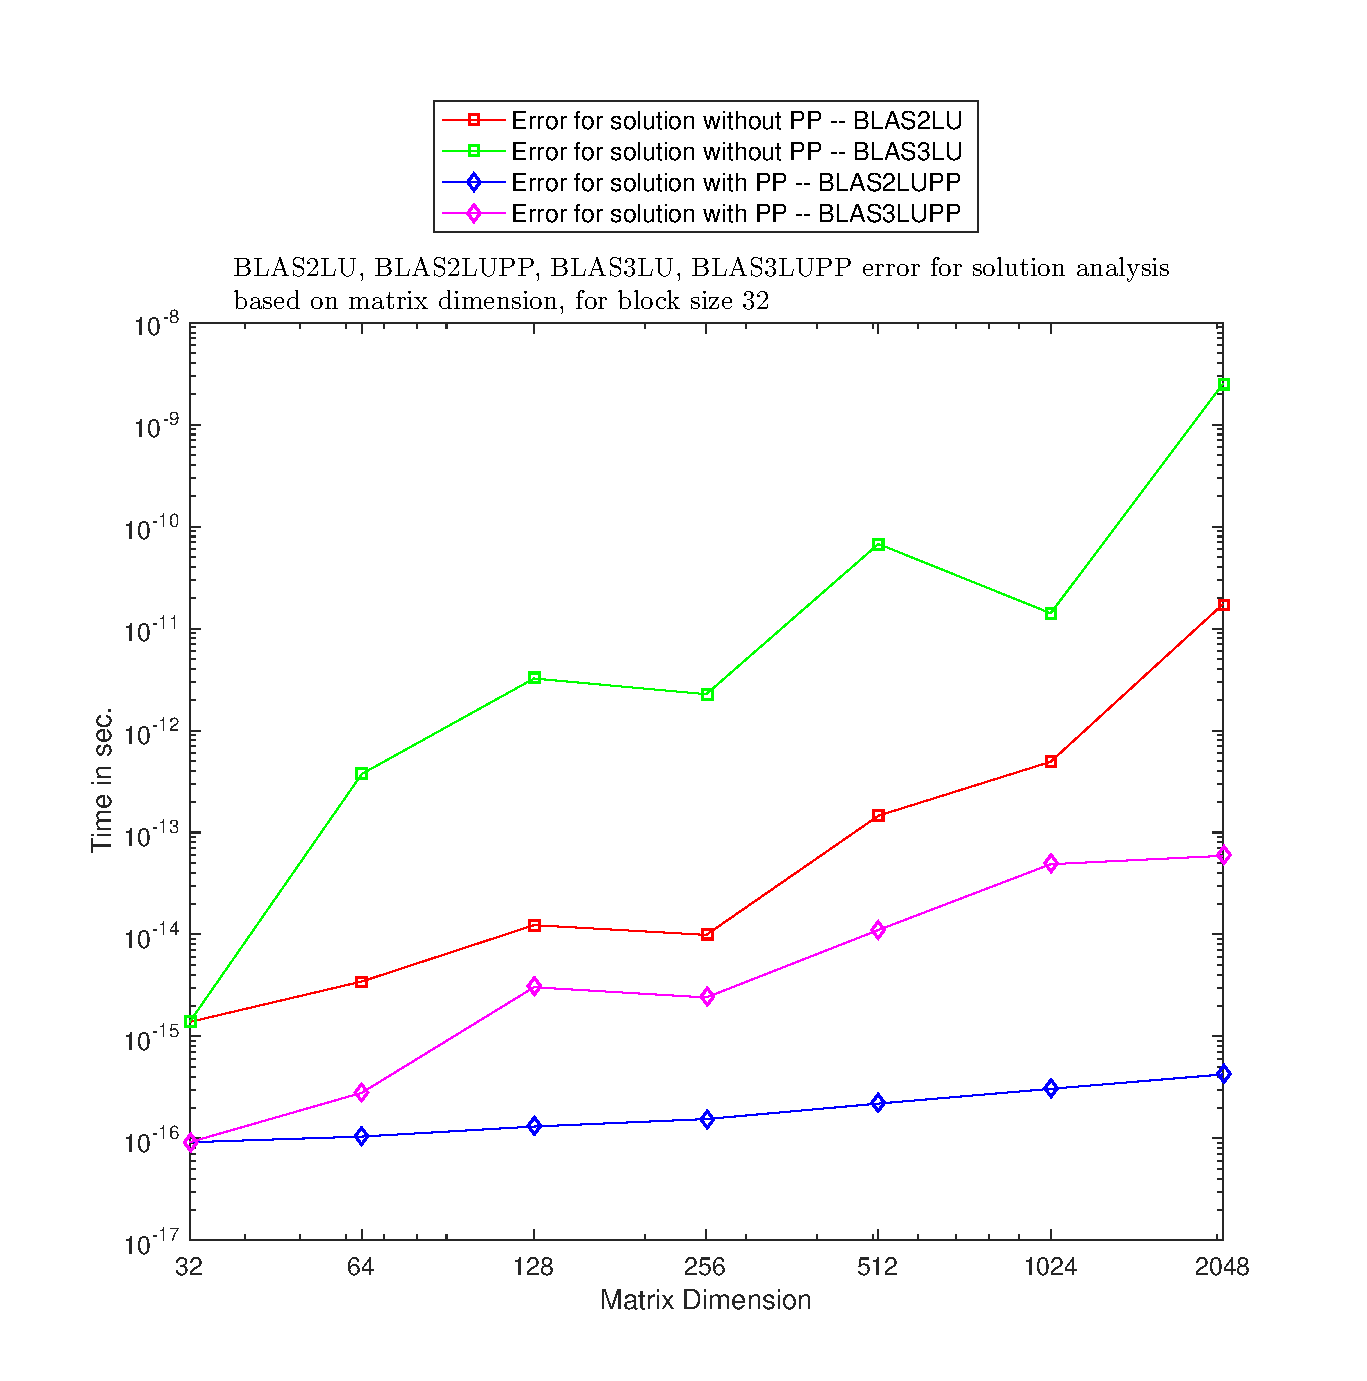
\includegraphics[width=1\columnwidth]{EPS/error_32.eps}
     \caption{Error for solution analysis based on matrix dimension, for block size 32}
     \label{graph:error_32}
     \end{figure}
     
     \begin{figure}[H]
     \centering
     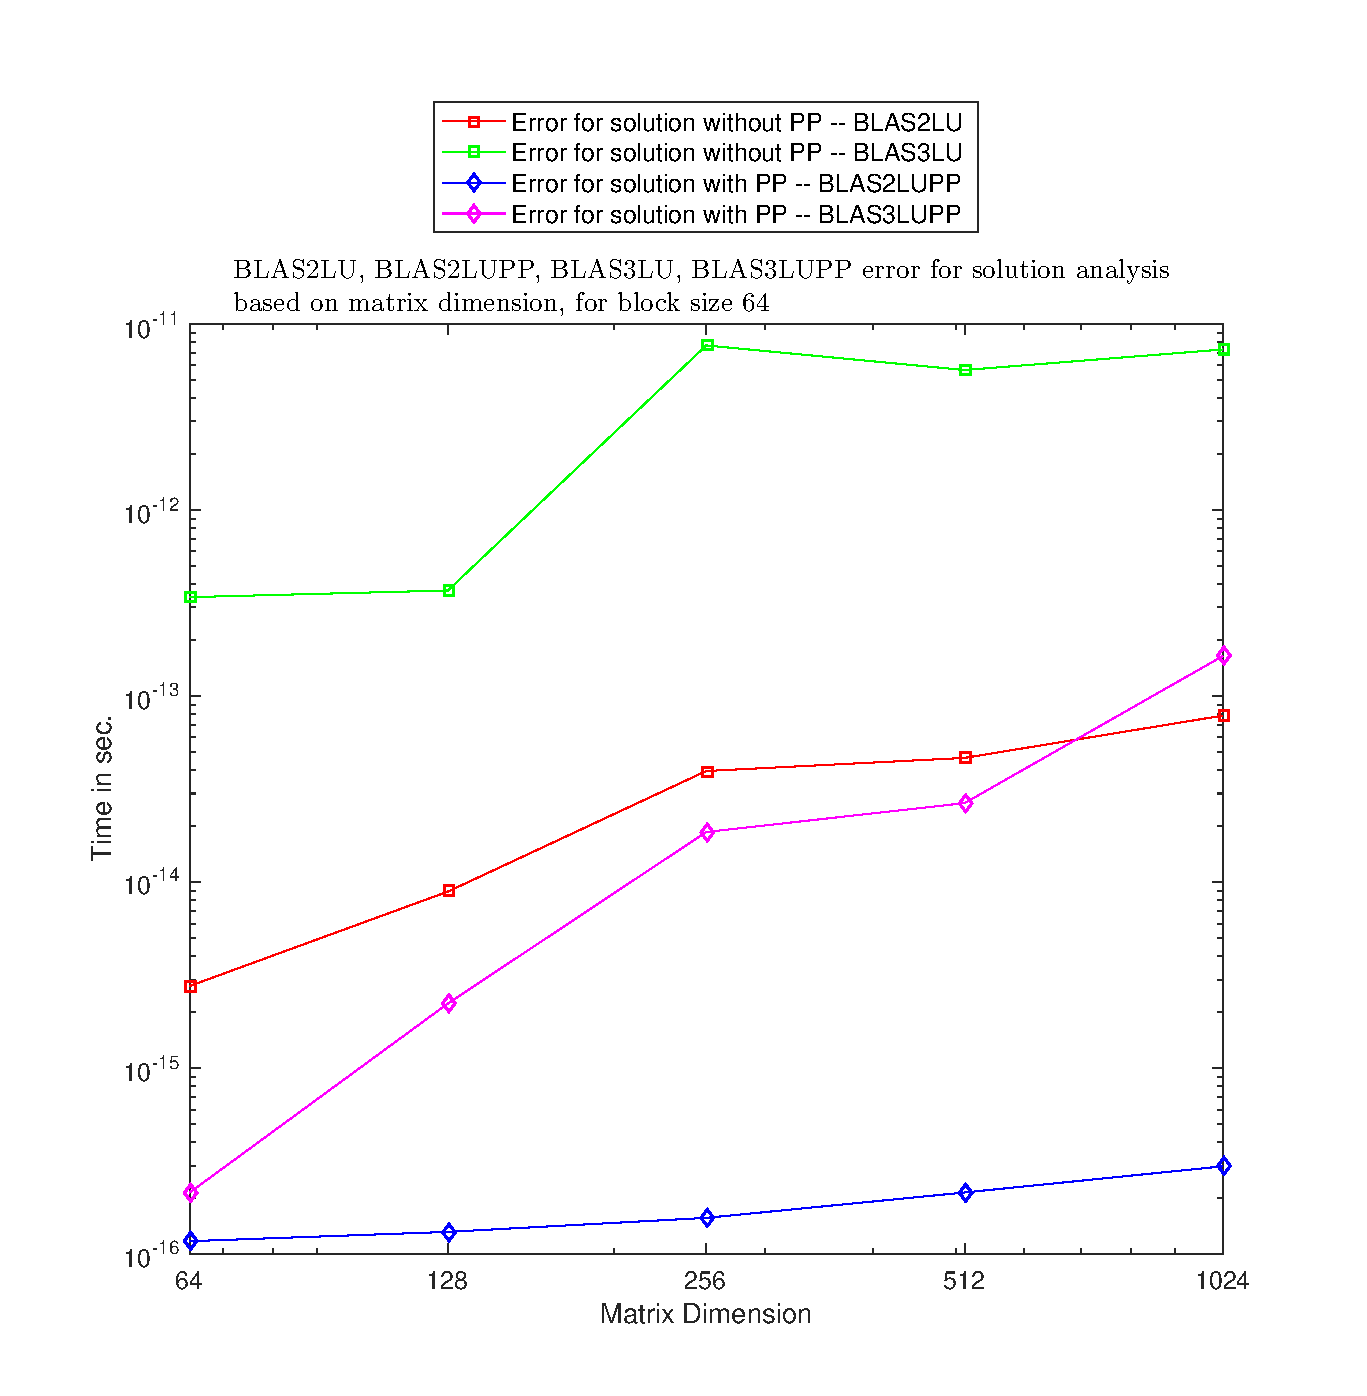
\includegraphics[width=1\columnwidth]{EPS/error_64.eps}
     \caption{Error for solution analysis based on matrix dimension, for block size 64}
     \label{graph:error_64}
     \end{figure}
     
     
     As predicted, the error value for algorithms that recur to Partial Pivot presents a value several orders of magnitude below the one presented by algorithms without Partial pivoting.
     
\section{Analysing the time for solutions based on algorithm and block dimension}  

Proved the algorithm correctness, we should analyse the total time for solution based on both the algorithm and the block dimension.\par 
Please denote that the block sizes were chosen based on the average CPU cache line size. \par The corresponding time analyse is shown in figures \ref{graph:time_32} and \ref{graph:time_64}. A relation between matrix block dimension and time for solution is presented on figure \ref{graph:time_32vs64}.

     \begin{figure}[H]
     \centering
     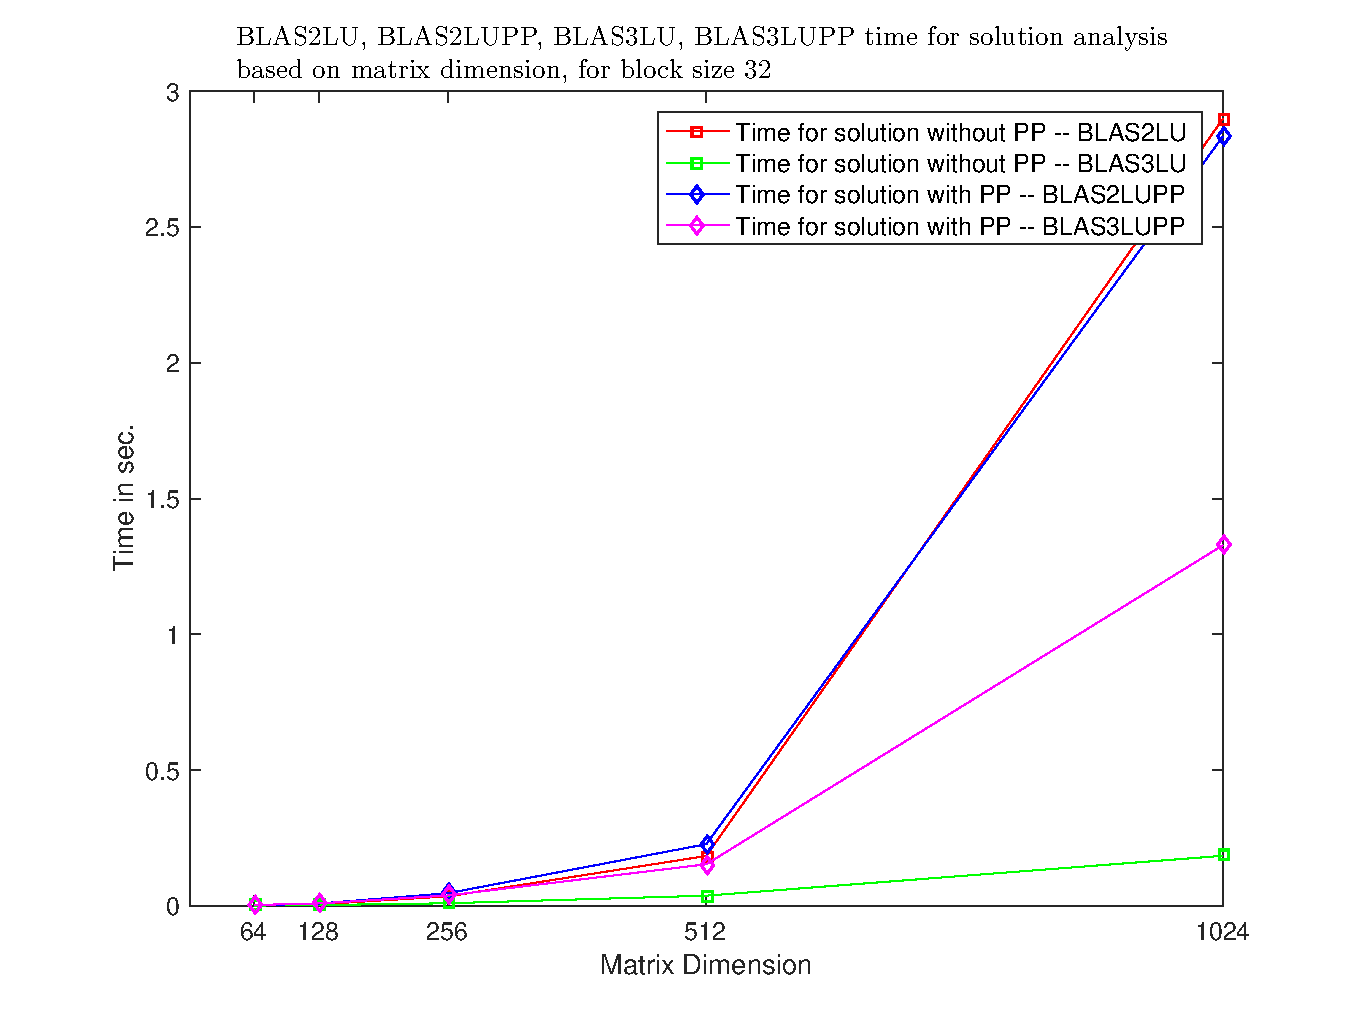
\includegraphics[width=1\columnwidth]{EPS/time_32.eps}
     \caption{Time for solution analysis based on matrix dimension, for block size 32}\label{graph:time_32}
     \end{figure}


    \begin{figure}[H]
     \centering
     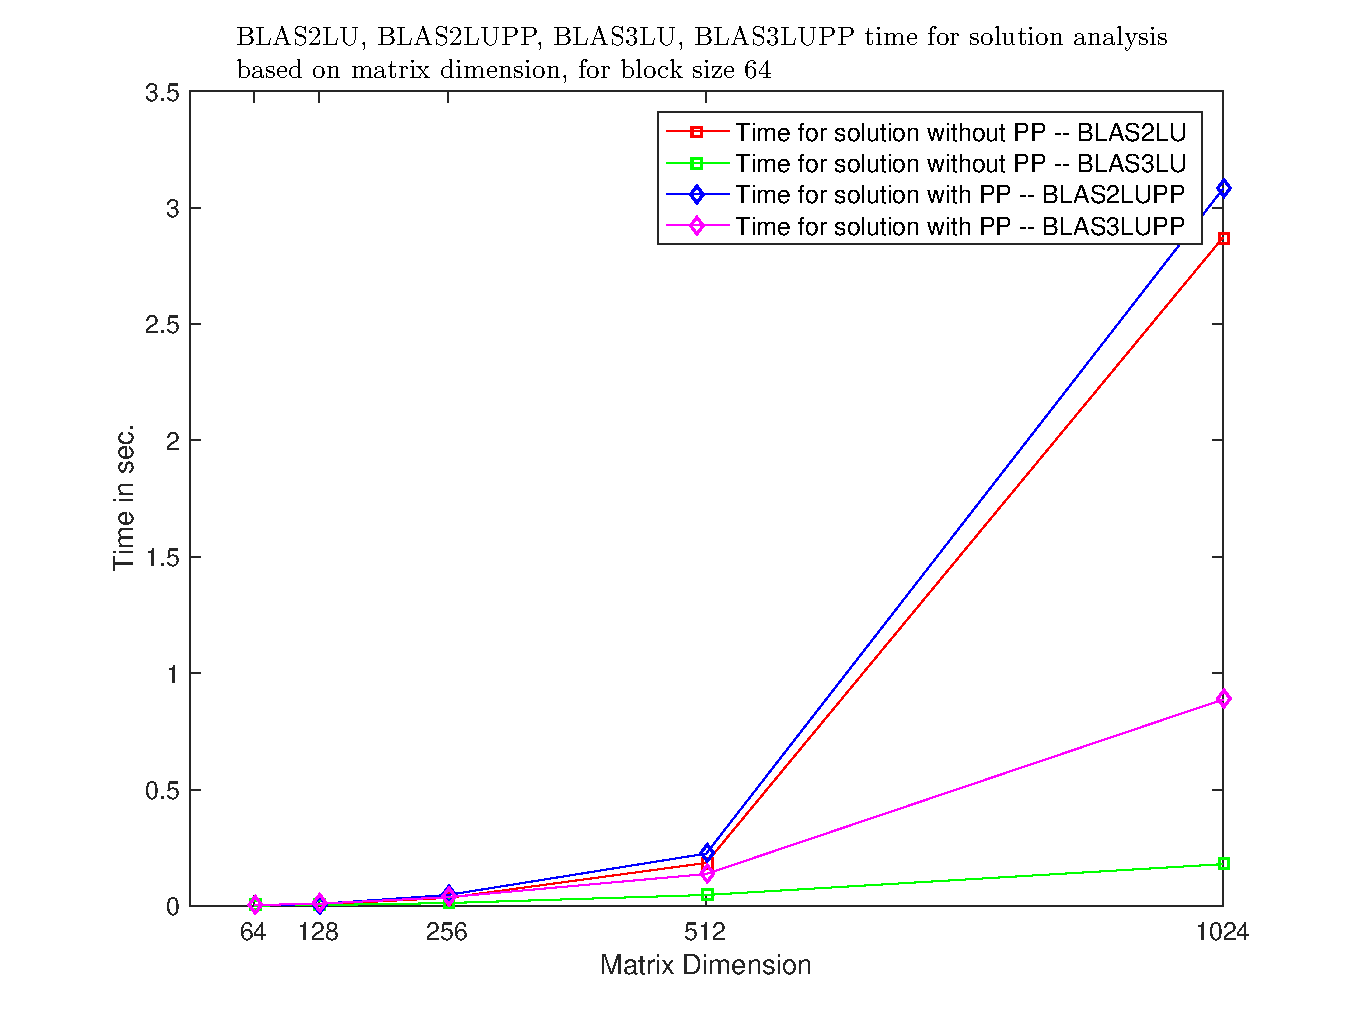
\includegraphics[width=1\columnwidth]{EPS/time_64.eps}
     \caption{Time for solution analysis based on matrix dimension, for block size 64}\label{graph:time_64}
     \end{figure}
  
  \begin{figure}[H]
     \centering
     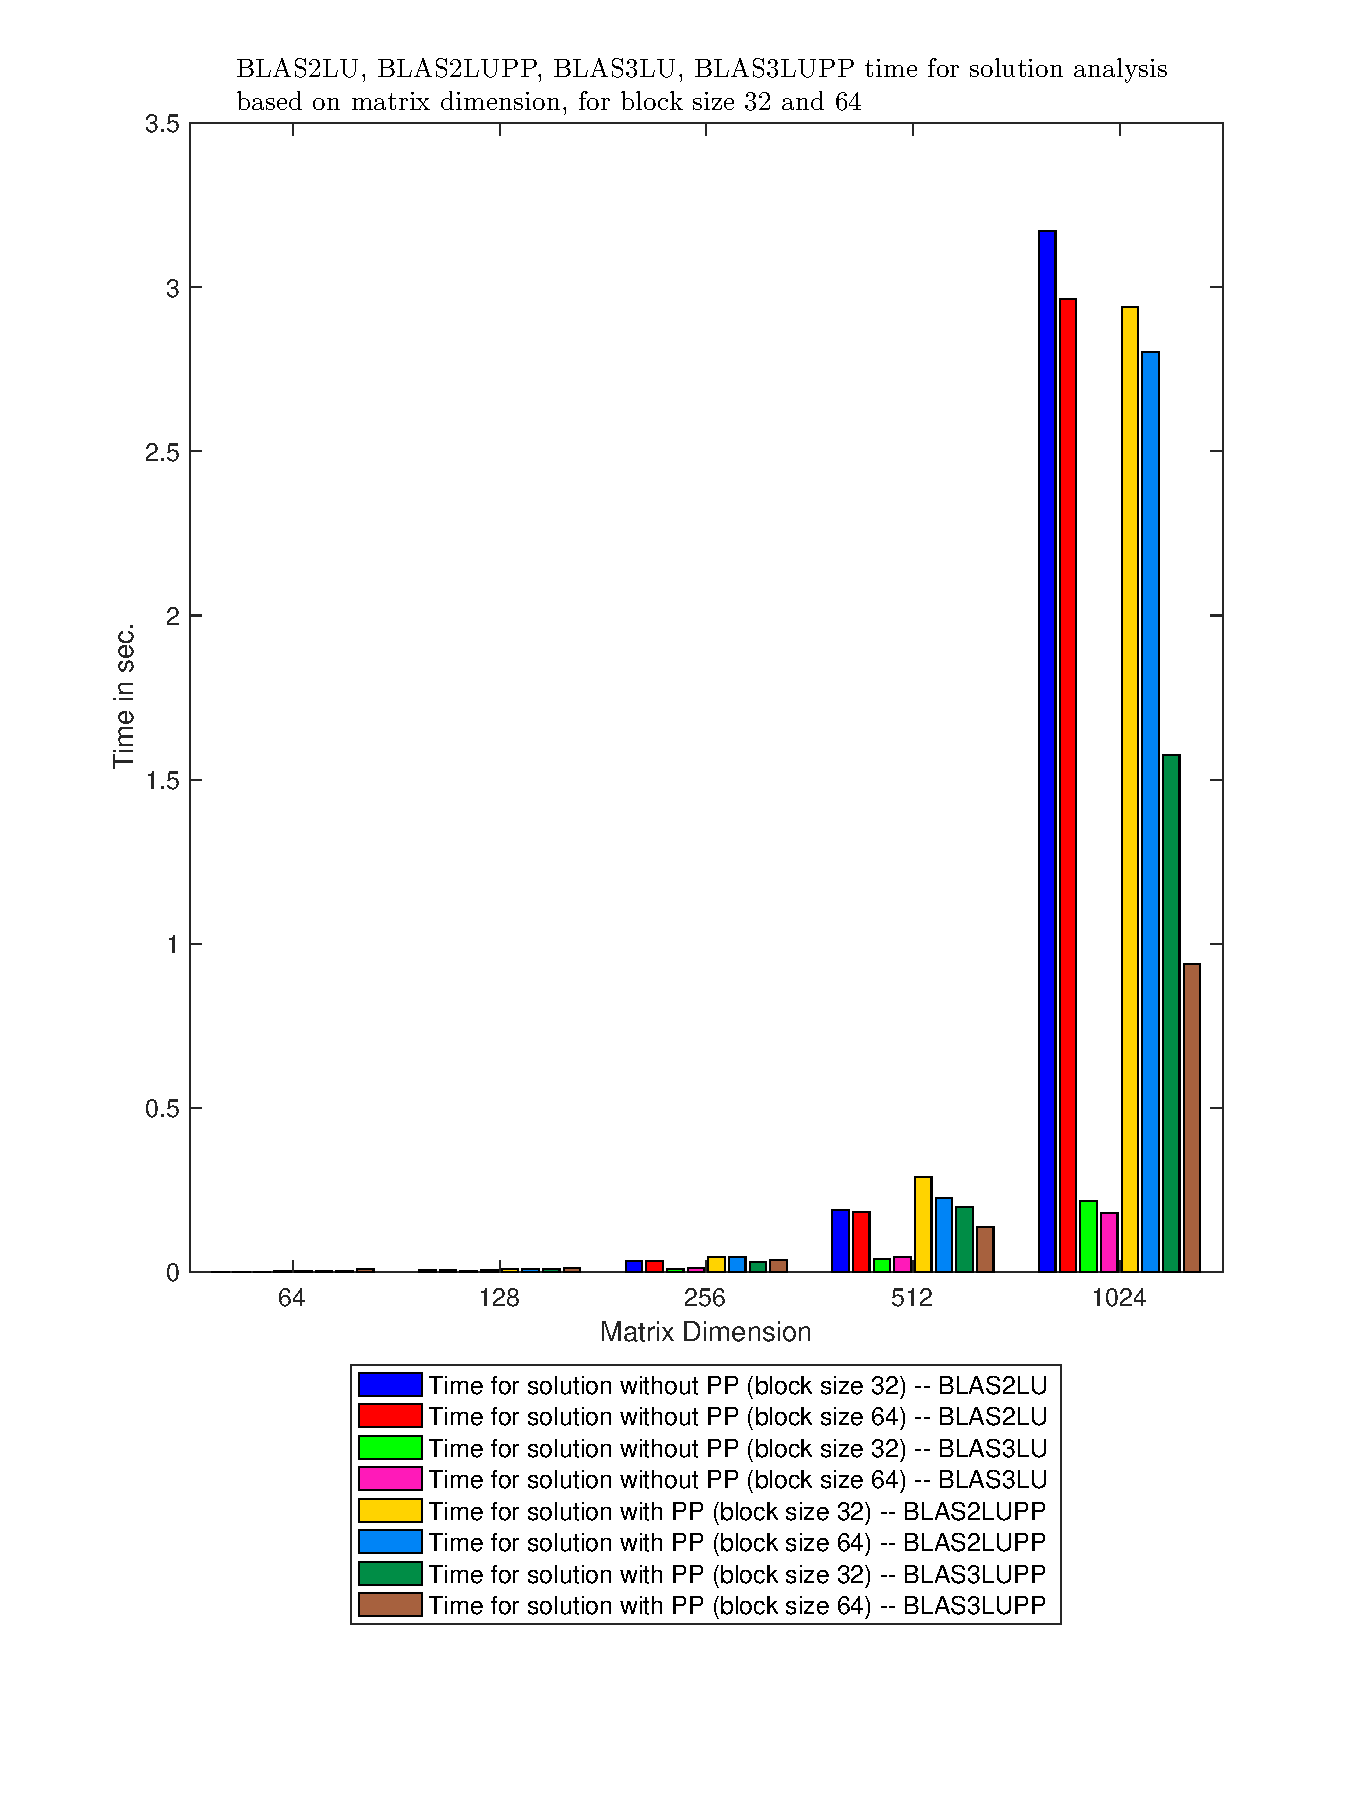
\includegraphics[width=1.1\columnwidth]{EPS/time_32vs64.eps}
     \caption{Time for solution analysis based on matrix dimension, for block size 32}\label{graph:time_32vs64}
     \end{figure}
     
     As we can visually infer, a block dimension of 32 produces better overall results in terms of time for solution. That was as expected result, since the computing platform used in the tests has as Cache line size of 32 Bytes.
  
\section{Conclusion}
As we can see, in the previous results, the relative error associated to the LU Factorisation with partial pivoting is less then the LU Factorisation without partial pivoting, because of this we can conclude that the LU Factorisation with partial pivoting is more accurate then FU Factorisation without partial pivoting.\par 

In terms of computation time the most expensive algorithms are the ones with partial pivoting. The total time for solution LU Factorisation with partial pivoting for BLAS2 has revealed to be the most expensive for block sizes of 32 and 64. \par 

As predicted, the usage of blocks in the algorithms, implied a better time for solution. \par

During this work we have come across with some problems, essentially on the implementation of the BLAS3 LU factorisation with partial pivoting. The bigger problem was the row permutations on this algorithm. We think that this difficulties were surpassed.


\nocite{*}
\bibliographystyle{abbrv}
\bibliography{ref.bib}
	

% that's all folks
\end{document}


